\section{Keys handling}

The issue of securely binding public keys to user identities is paramount in both asymmetric encryption and digital signatures.
Failure to authenticate public keys can lead to serious consequences, including susceptibility to Man-in-the-Middle attacks in asymmetric encryption and the potential for unauthorized signature generation by malicious actors.

To ensure the authenticity of public keys, an additional layer of verification, often in the form of another signature, is necessary. 
This additional signature serves as a guarantee of the legitimacy of the public-key and identity pairing. 
To facilitate this process, there is a requirement for a standardized format for distributing these signed pairs securely across systems.

\subsection{Digital certificates}
Digital certificates serve the purpose of associating a public key with a specific identity. 
This identity can be represented as an ASCII string for human interpretation or as either the Canonical Name (CNAME) or IP address for machine understanding. 
Additionally, these certificates outline the intended usage of the public key they contain, eliminating any potential ambiguities when a key format is suitable for both encryption and signature algorithms.

Furthermore, digital certificates include a designated time frame during which they are deemed valid. 

\subsection{Certification authorities}
The certificates are signed by a trusted third party, known as the Certificate Authority (CA). 
This CA's public key is authenticated using another certificate. 
This process extends even to self-signed certificates, which must be trusted beforehand.
\begin{figure}[H]
    \centering
    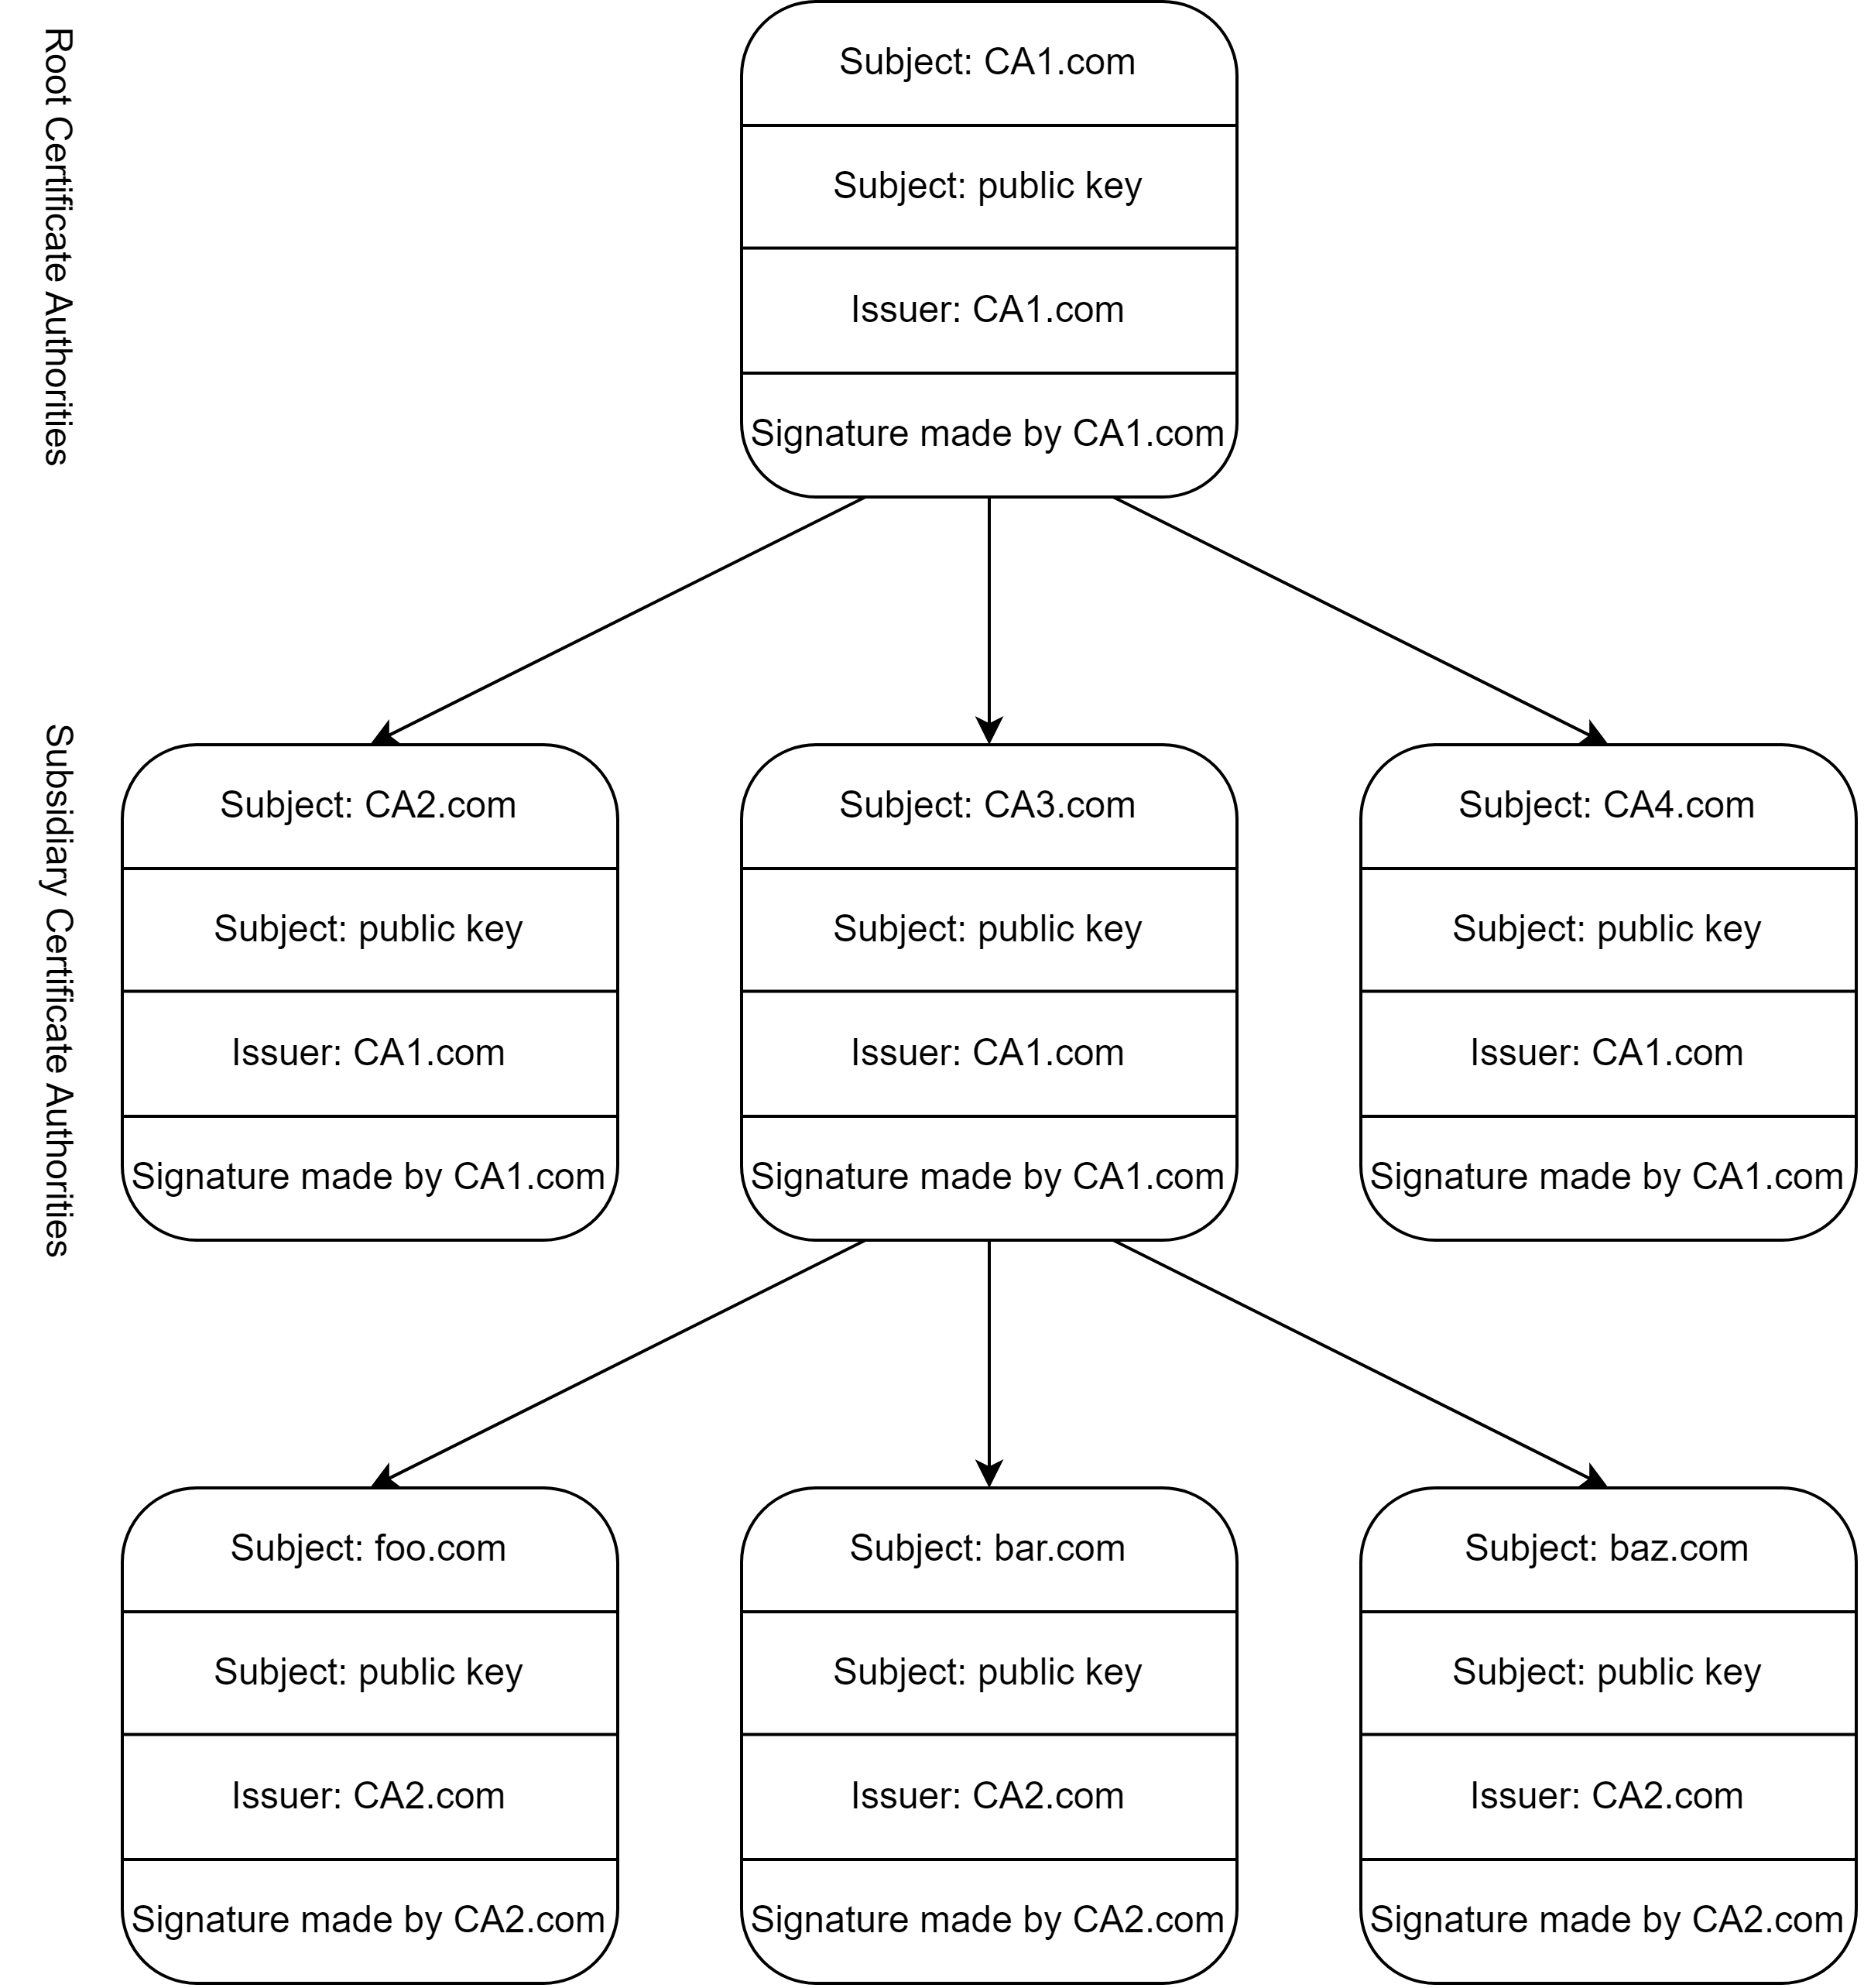
\includegraphics[width=0.5\linewidth]{images/ca.png}
    \caption{Certificate authorities hierarchy}
\end{figure}